\documentclass{article}
\usepackage[utf8]{inputenc}
\setlength{\parskip}{1em}
\usepackage{subcaption}


\title{Chapter 3}
\author{Jonathan S. Abrahams }
\date{October 2019}

\usepackage{natbib}
\usepackage{graphicx}

\begin{document}

\maketitle

\section{Introduction}

%People have done GWAS on TB before. They mostly stick to SNPs and short indels.

%General GWAS on TB for AR:
%https://www.nature.com/articles/s41467-019-10110-6
%https://www.nature.com/articles/s41598-019-51812-7
%Studies somewhat taking into account genomic variation outside of SNPs:


%Studies that directly studied gene presence or absence and their association with resistance:

%Identified only one genomic deletion that was associated. No relationship to our data.

%https://www.nature.com/articles/s41588-017-0029-0#Sec2

%We used a subsection of this data:

%https://www.ncbi.nlm.nih.gov/pmc/articles/PMC4579482/#sec1
\begin{figure}[h!]
\centering

\includegraphics[scale=1.7]{universe}
\caption{The Universe}
\label{fig:universe}
\end{figure}

\section{Results}

There is a plethora of tools to undertake GWAS in both eukaryotic and prokaryotic organisms, most tools are based on detecting SNVs whilst some also analyse the presence or absence of whole genes. However there has been, to our knowledge, no capacity to study structural variants beyond deletions using a GWAS framework. We therefore developed a suite of methods to process SV data into a format that is compatible with GWAS tools and then tested them on a dataset.






\subsection{Structural variations as an effective genotype}


\subsubsection{Read depth based duplications as a genotype for GWAS}

As shown previously, read depth can be a reliable proxy for copy number. Therefore, the previously generated dataset, with a copy number assigned to each gene of each strain, was inputted to pySEER as a matrix. This was possible on pySEER as it can take a binary matrix, intended for the study of pangenomes, as input. However this meant that the CNV data had to be binary and genes with a copy number equal to or less than 1 were set as 0 and genes with a copy number greater than 1 were set to 1.


In order to use SVs as the ‘genotype’ in the ‘genotype-phenotype’ link that GWAS aims to establish, it was first necessary to prove the concept in a proof of concept experiment. In a standard GWAS experiment, phenotypes (such as `MIC $\leq$ 128ug' or `Can metabalise lactose') are often used in a binary format-the outcomes are logged as a zero (0) or one (1). The easiest genotype-phenotype link to discover using GWAS is the 'perfect link' in which a single genotype wholly and consistently is associated with a specific phenotype. To undertake a proof of concept experiment a 'perfect link' phenotype was emulated: the strains containing duplications in Network 1 were given the phenotype of 1 and all other strains were given the phenotype of 0 in this model phenotype. The `genotype' used was the copy number predictions for each gene in each strain.





\begin{figure}[h!]
\centering
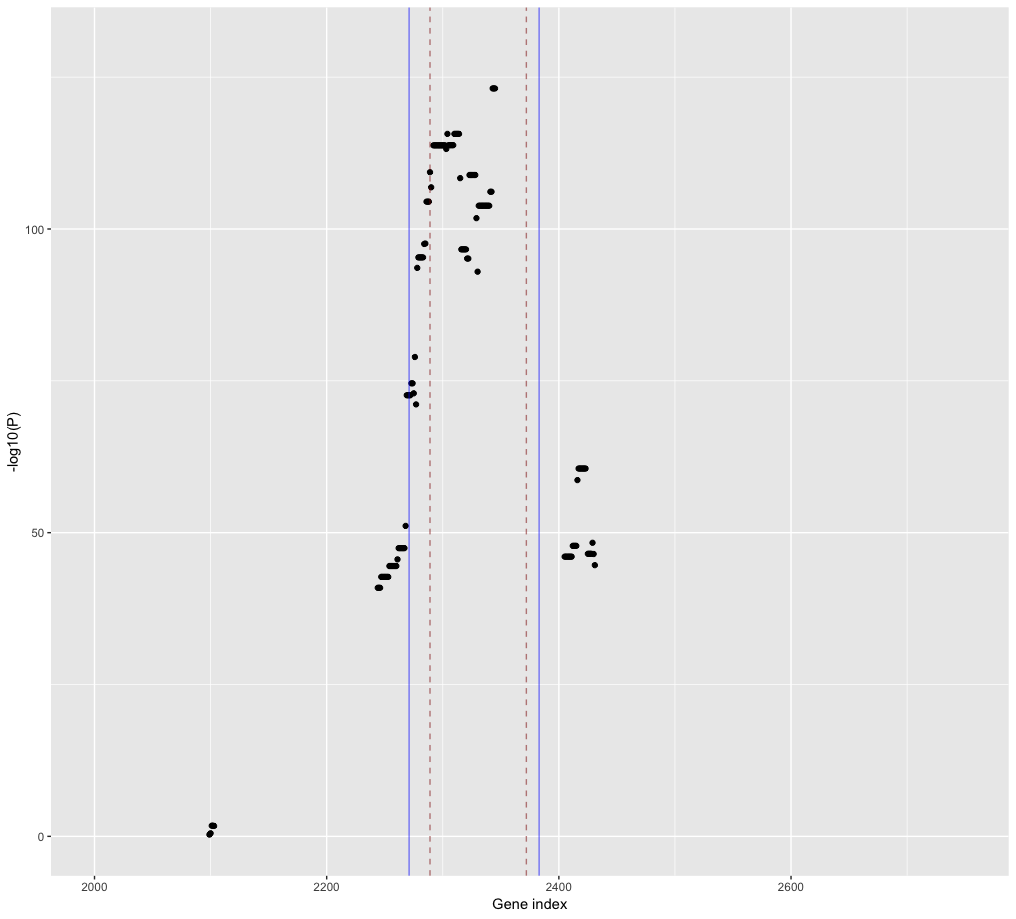
\includegraphics[width=\textwidth]{just core.png}
\caption{Manhatten plot demonstrating a genotype-phenotype link can be established using Duplications and a 'perfect' phenotype. Red line indicates Mean start and end of the duplication in Network 1 and blue line indicates the core of the network. }
\label{fig:Manhatten_1}
\end{figure}




Running a GWAS with the emulated 'perfect link' genotype-phenotype data resulted in the duplicated genes being significantly associated with the 'perfect link' phenotype (Figure \ref{fig:Manhatten_1}). Therefore It could be proved that duplications,in principle, could be used as a 'genotype' in GWAS. In this contrived experiment,however, there is nothing but the correct signal and therefore this represents an unrealistic scenario. With less contrived phenotypes, therefore, such warnings would likely be less frequent.

\clearpage
\begin{figure}[h!]
\centering
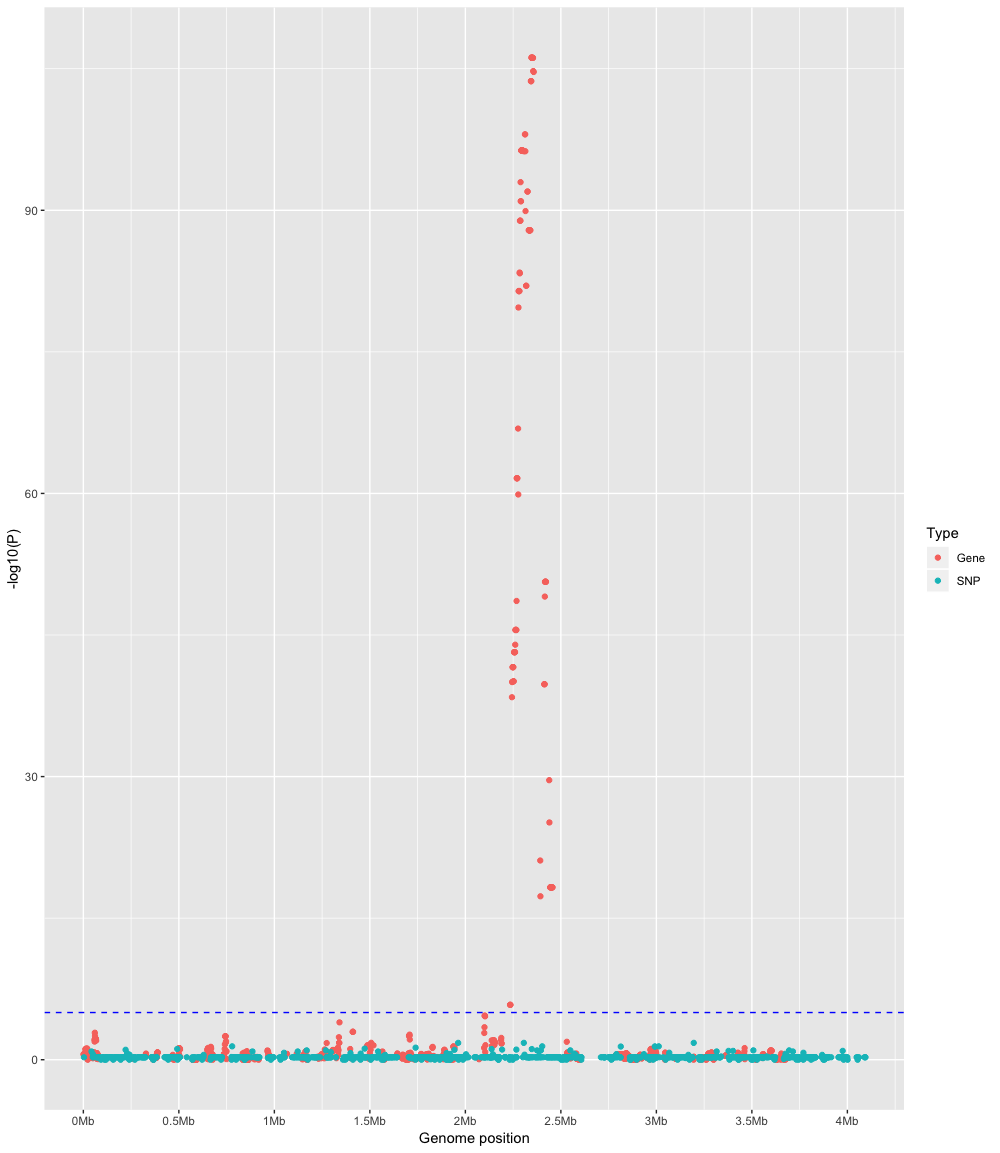
\includegraphics[width=\textwidth]{Chapter_3/Rplot15.png}
\caption{Manhatten plot demonstrating a genotype-phenotype link can be established using duplications,deletions and SNPs and a 'perfect' phenotype.}
\label{fig:Manhatten_1}
\end{figure}
\clearpage

We reran the analysis with the other duplications,deletions and SNPs in the data included. The association still persisted.
\clearpage

%BP is highly highly clonal.

%Whats nice about duplications is that they have practically no phylogenetic signal (See chapter 2 ASR).

%This means they are independent to the highly clonal population structure of BP, potentially posing them as a perfect trait to investigate using gwas.

%We investigated how robust they were to the underlying population structure (somehow...)
	%Population structure is the the tree. Mutate the tree to

%We could demonstrate that this was independent of underlying structure but we wanted to see how regular SNPs would fare.

%We therefore showed there was extremely high linkage between SNPs in pertussis with an LD plot

%We then did a GWAS using faked phenotypes for 2 things: FIrstly we did the chinese resistance ting, then we chose something else relevant.


%We then switched to K-mers. We wanted to study gene order in combination with all other effects, using a unified system. If duplications were easily solved like this, it would also be useful.
\subsection{Using gene order as a genotype for GWAS}

We wanted to see if gene order, as specified in resolved genomes, could be used as genetic material for GWAS.

Bp is fantastic for this. Gene order changes frequently, over short evolutionary timescales.

\begin{figure}[h!]
\centering
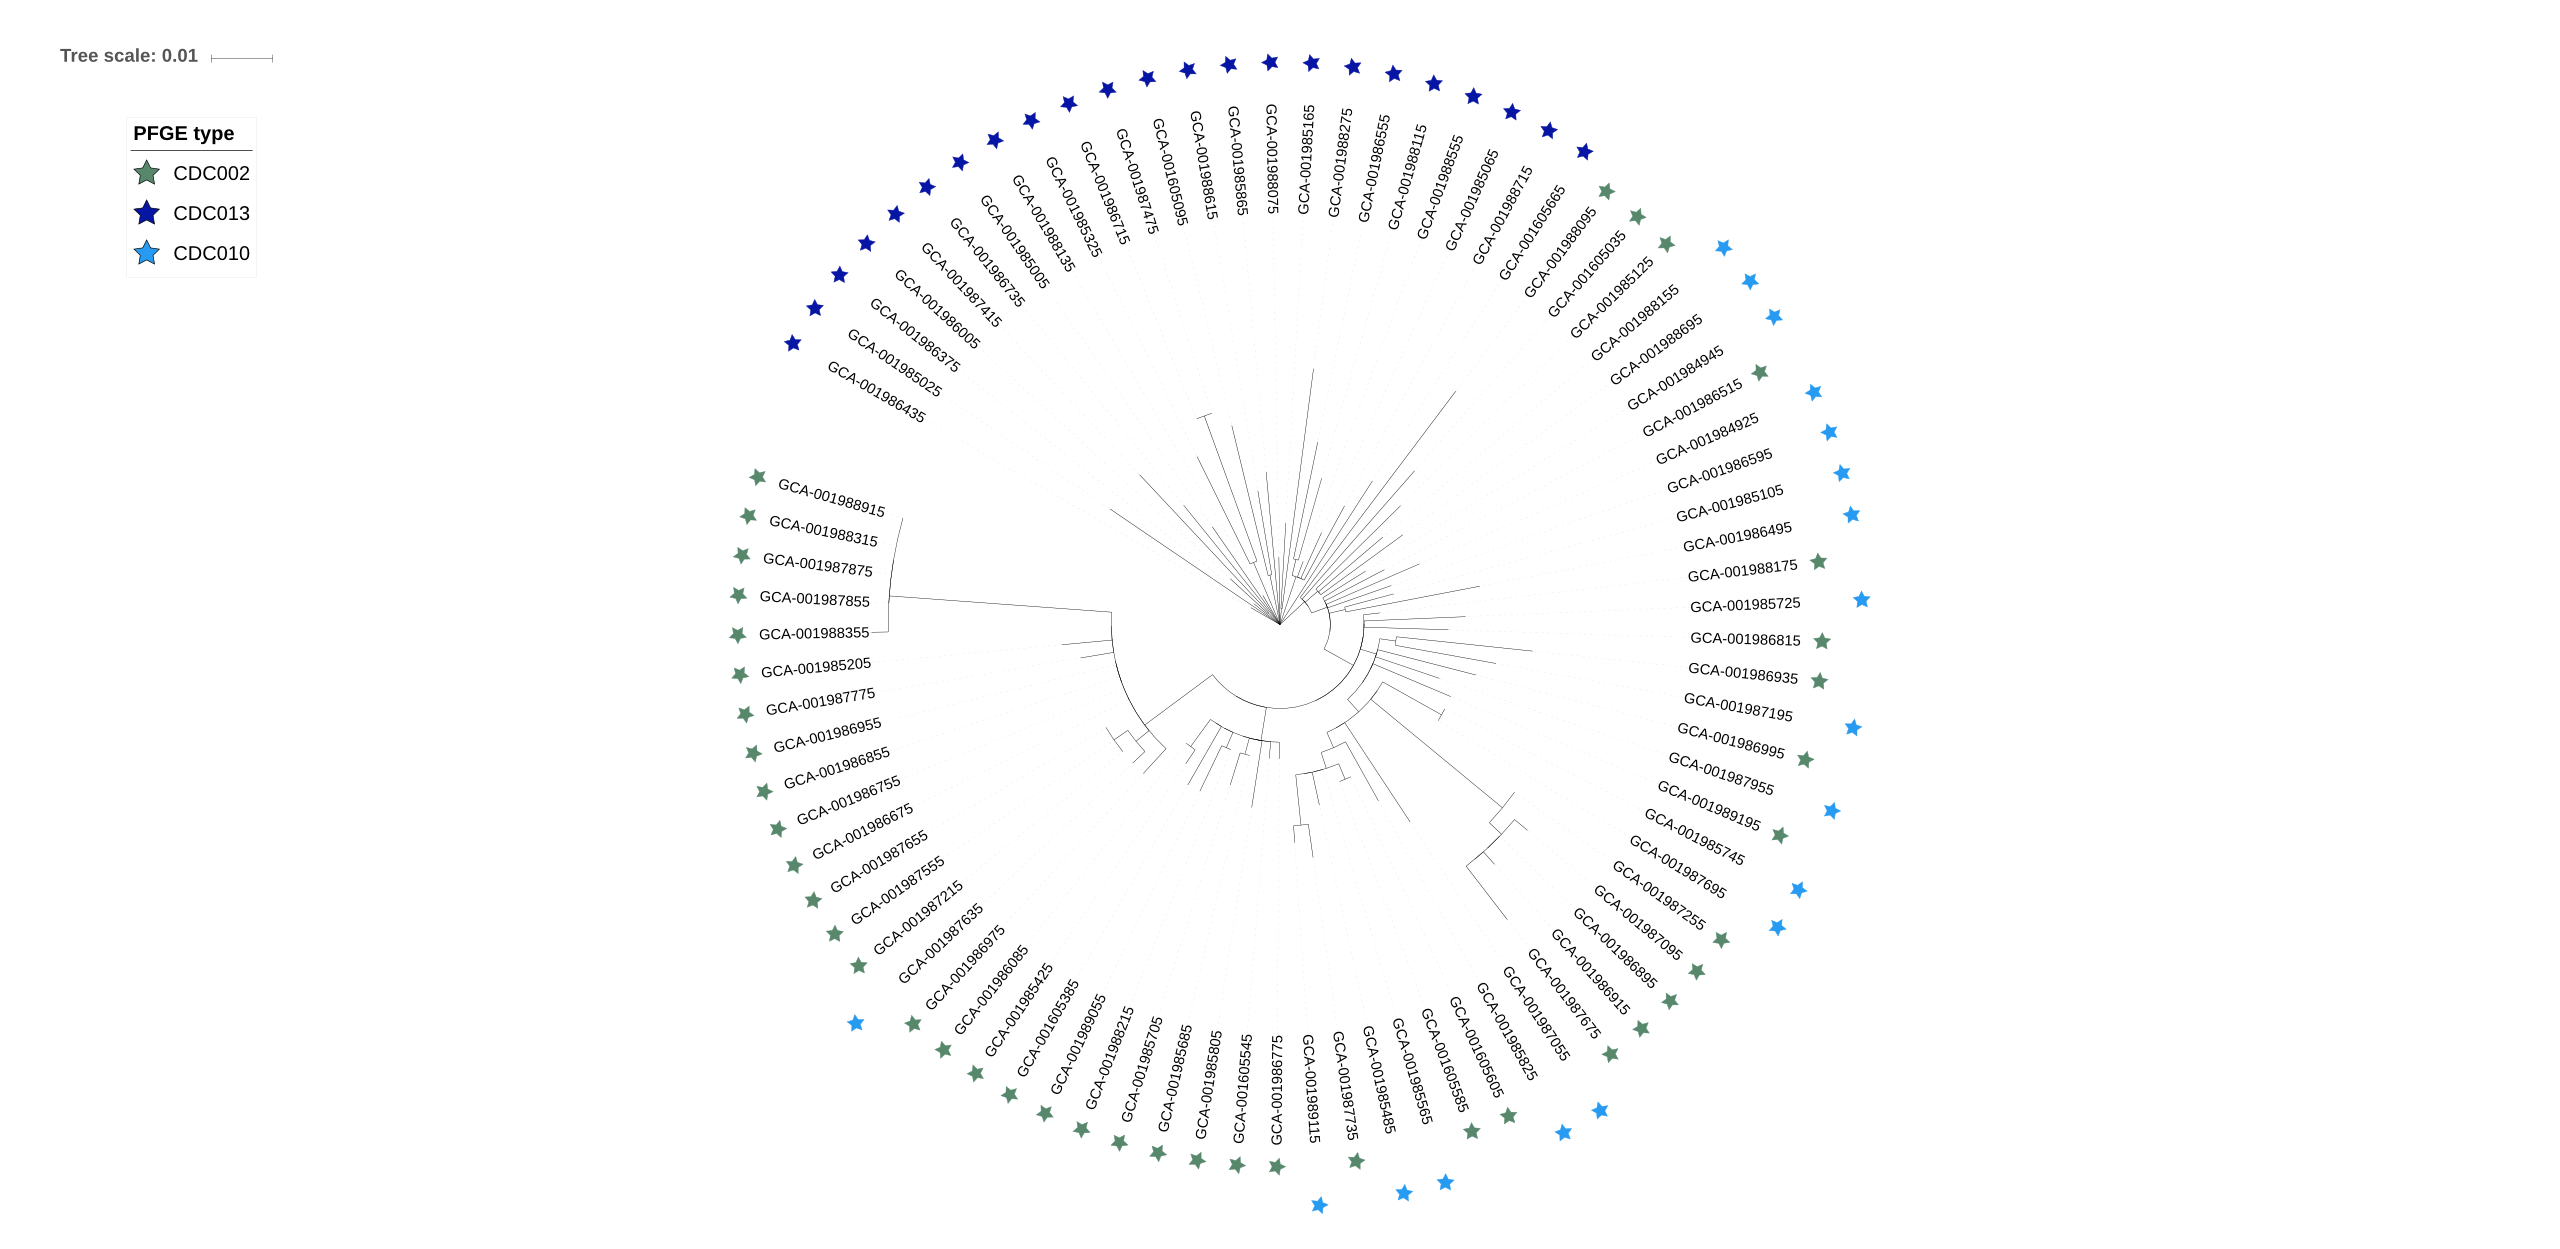
\includegraphics[width=\textwidth{}]{PFGE_tree.png}
\caption{PFGE types are homoplasic}
\label{fig:PFGE_tree}
\end{figure}

We therefore depleted the genome of repeat elements in order to produce informative kmers of reasonable length.

It was also possible to produce ultra long kmers, however, whilst useful in pertussis, their use outside the species, with more diverse genomes, would be limited. The more generic methodology, of depleting repeat regions, was pursued.




\end{document}
